\documentclass[10pt]{beamer}

\mode<presentation> {

\usetheme[compress]{Szeged}
}

\usepackage{graphicx} 
\usepackage{booktabs} 
\usepackage{bibentry}
\usepackage{color}
\usepackage{setspace}
\usepackage{transparent}

% The line below is what I talked about that makes all
% items in a list into overlays
%\beamerdefaultoverlayspecification{<+->}

\newcommand{\tc}[1]{$\backslash$\texttt{#1}}

\title{Search Optimization for JPEG Quantization Tables}
\subtitle{using a Decision Tree Learning Approach}
\author{Sharon Gieske\\6167667\\~\\}
\institute[UvA] % Your institution as it will appear on the bottom of every slide, may be shorthand to save space
{
Supervisors: Zeno Geradts (NFI)\\~\\
Master System and Network Engineering\\
University of Amsterdam \\
}
\date{2014-07-02} % Date, can be changed to a custom date

\begin{document}
\bibliographystyle{plain}

\frame{
\maketitle
}
\frame{
\frametitle{Table of Contents}
\tableofcontents
}

\section[Introduction]{Introduction}

\subsection{Motivation}
\begin{frame}
\frametitle{Motivation}~\\
\begin{itemize}
\item Growing popularity for taking pictures
\item Digital images often recovered in forensic investigations
\item Identify origin of images to a specific camera or common source
\item Large sets of images are retrieved
%forecast of 86 million cameras sold in 2013
%\item 250 billion photos uploaded to Facebook, 20 billion photos on Instagram
\end{itemize}
~\\
\textbf{Camera Identification}:
\begin{itemize}
\item Intrinsic features of camera hardware give more reliable results\cite{van2007survey}
\item Sensor Imperfections, CFA Interpolation, Image Features
\end{itemize} 
\end{frame}

\begin{frame}
\frametitle{JPEG quantization tables}
JPEG compression:
\begin{itemize}
\item RGB to Luminance-Chrominance colour space
\item Splitting into two 8$\times$8 blocks
\item Discrete Cosine Transform (spatial domain $\rightarrow$ frequency domain)
\item Compression ratio
\item Correlated to camera make/model
\end{itemize}
~\\
\textit{`..is reasonably effective at narrowing the source of an image to a single camera make and model or to
a small set of possible cameras.'}\cite{farid1}
\end{frame}

\subsection{Decision tree learning algorithm}
\begin{frame}
\frametitle{Decision tree learning algorithm}
Camera identification problem $\rightarrow$ pattern recognition problem:\\
\begin{itemize}
\item map feature set to corresponding label
\end{itemize}
~\\
Decision tree learning algorithm:
\begin{itemize}
\item Rule based, generates best splits
\item Simple to interpret / human readable
\end{itemize}
\end{frame}

\subsection{Research Question}
\begin{frame}
\frametitle{Research Question}
\begin{center}
\textbf{\Large Can searching through JPEG quantization tables be optimized with the use of decision tree learning?} \\ ~\\
\end{center}
~\\
Subquestions:
\begin{enumerate}
\item Can identifiable parameters be found in JPEG quantization tables?
\item What is the performance of decision tree learning with JPEG quantization tables?
\end{enumerate}
\end{frame}




\section[Approach]{Approach}
\subsection{Overview}
\begin{frame}
\frametitle{Overview}
\begin{enumerate}
\item Extract quantization tables from images
\item Generate feature set
\item Train decision tree classifier (make/model) 
\item Evaluate classifications
\item Compare against method using hash database
\end{enumerate}
\end{frame}

\subsection{Data Preprocessing and Training}
\begin{frame}
\frametitle{Data Preprocessing and Training}
\textbf{1. Extract quantization tables from images}
\begin{itemize}
\item Unix command: djpeg
\end{itemize}
\textbf{2. Generate feature set}
\begin{itemize}
\item Add features: sum, min, max, mean, median, var, std
\item Run feature selection
\end{itemize}
\textbf{3. Train decision tree classifier}
\begin{itemize}
\item CART: combines classification and regression trees
% continous: regression, categorial classification
\end{itemize}
\end{frame}


\subsection{Evaluation}
\begin{frame}
\frametitle{Evaluation}
\textbf{4. Evaluate with weighted F$_\beta$-score}
\begin{itemize}
\item Recall is more important: $\beta$ = 2
\end{itemize}
\begin{equation}
F_\beta = 1 + \beta^{2} * \frac{precision * recall}{(\beta^{2} *precision) + recall}
\end{equation}
~\\
\textbf{5. Compare against method using hash database}
\begin{itemize}
\item Database of hashed quantization tables
\begin{itemize}
\item 1$\rightarrow$1 mapping
\item 1$\rightarrow$n mapping
\end{itemize}
\item Use same training and validation data
\end{itemize}
\end{frame}

\section[Results]{Results}
\begin{frame}
\frametitle{Results}
Dataset:
\begin{itemize}
\item 45,666 images (NFI \& Dresden Image Database)
\item 41 camera models
\item 19 camera makes
\item 1,016 unique quantization tables
\end{itemize}
~\\Identifiable parameters: 50 out of 128 \\
603 nodes, depth of 26
\begin{figure}
   \fbox{
   	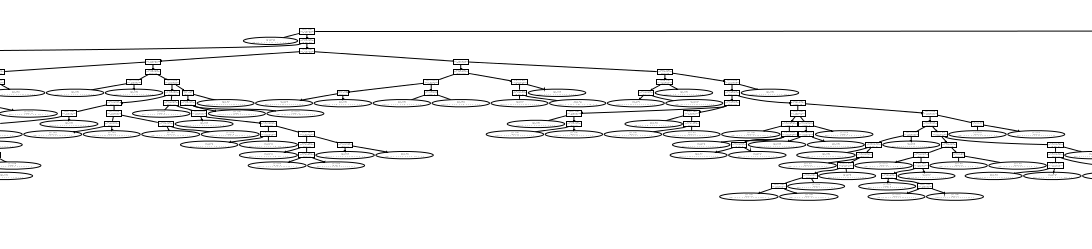
\includegraphics[scale=.25]{decisiontree_quarter.png}
   	}
   \caption{Partial Decision Tree}
\end{figure}
\end{frame}


\begin{frame}
\frametitle{Zoom in: F2-score for camera make}
\begin{table}
\begin{tabular}{| l | r | c | l | r |}
\hline
\textbf{Make} & \textbf{F2} &  & \textbf{Make} & \textbf{F2} \\
\hline
Kodak & 99 \% & & Praktica & 43 \% \\
Ricoh & 94 \% & & Nikon & 86 \% \\
Panasonic & 79 \% & & Casio & 99 \% \\
PS & 100 \% & & Canon & 98 \% \\
Olympus & 64 \% & & Logitech & 100 \%\\
Sony & 58 \% & & Motorola & 100 \% \\
Agfa & 78 \% & & Epson & 100 \% \\
Rollei & 84 \% & & BlackBerry & 100 \% \\
Samsung & 67 \% & & Pentax & 80 \% \\
FujiFilm & 96 \% & &  & \\
\hline
\end{tabular}
\caption{F2-score for camera make}
\end{table}

\end{frame}

\begin{frame}
\frametitle{Decision tree vs Hash databases}
~\\\begin{itemize}
\item 5-Fold Stratified Cross Validation
\item 80 \% Train set, 20 \% Validation set
\end{itemize}

\begin{table}
\begin{small}
\begin{tabular}{| c| c| c| c|}
\hline
Algorithm & Precision & Recall & F2-score\\
\hline
Hash (1-1) & 79 \% & 68 \% & 68 \%\\
Hash (1-n) & 50 \% & 99 \% & 83 \%\\
Decision tree & 90 \% & 89 \% & 89 \% \\
\hline
\end{tabular}
\caption{Camera Make Identification}
\end{small}
\end{table}
%1300 tables which have mutliple possibilities and thereby increasing the search space for fuurther research
\begin{table}
\begin{small}

\begin{tabular}{| c| c| c| c|}
\hline
Algorithm & Precision & Recall & F2-score\\
\hline
Hash (1-1) & 54 \% & 39 \% & 37 \%\\
Hash (1-n) & 50 \% & 98 \% & 83 \%\\
Decision tree & 78 \% & 82 \% & 80 \% \\
\hline
\end{tabular}
\caption{Camera Model Identification}
\end{small}

\end{table}
\end{frame}



\begin{frame}
\frametitle{Discussion}
\begin{itemize}
\item Both methods are prone for overfitting
\item Hash database holds larger search space
\item Training hash database is quicker
\end{itemize}
\end{frame}


\section{Conclusion}
\begin{frame}
\frametitle{Conclusions}
\begin{itemize}
\item Parameters can be reduced to 50
\item Decision tree classifier gains better F2-score of 89\% (make)
\item 1$\rightarrow$N hash database gains better F2-score of 83\% (model)\\~\\
\item Decision tree classifier is more flexible, reduces search space, but harder to train than 1$\rightarrow$N hash database
\end{itemize}
~\\\textbf{Future work}:
\begin{itemize}
\item Compare to other learning algorithms
\begin{itemize}
\item Naive Bayes
\end{itemize}
\item Extend feature set
\end{itemize}
\end{frame}

\section[Questions]{Questions}
\begin{frame}
~ \\~ \\~ \\
\begin{center}\Huge Questions? \end{center} 
\end{frame}

\begin{frame}[allowframebreaks]
        \frametitle{References}
        \bibliographystyle{unsrt}
        \bibliography{../report/scriptie_literatuur.bib}
\end{frame}


\end{document}